\documentclass[fleqn,10pt]{article}




\usepackage[left=2cm,right=2cm,
			top=1.25cm,
			bottom=2.25cm,%
			headheight=11pt,%
			letterpaper]{geometry}
			
\frenchspacing			

\nonstopmode






\usepackage{lmodern}
\usepackage[T1]{fontenc}
\usepackage[utf8]{inputenc}

\usepackage[sfdefault]{roboto}
\fontseries{t}\selectfont

\usepackage{noweb}

\usepackage{multicol}
\usepackage{fancyhdr}
\usepackage{blindtext,graphicx}
\usepackage[absolute]{textpos}
%\usepackage[parfill]{parskip}
\usepackage{parskip}
\setlength{\parskip}{\baselineskip}

\usepackage[colorlinks=true,citecolor=brown]{hyperref}
\usepackage{gensymb}
\usepackage{csquotes}
\usepackage{amsmath}
\usepackage{fontawesome}
\usepackage{orcidlink}
\usepackage{standalone}
\usepackage{pdfpages}
\usepackage{subfiles}
\usepackage{svg}
\listfiles
% it would be best if this was a list of directories 
\svgpath{{../biology/simulation/GROMACS/BUMPy_bilayer/data/}{../electronics/propagation/} {../math/mathematica/output/}}

\usepackage{sidecap}
\usepackage{float}
\usepackage{amssymb}
\usepackage{textcomp}
\usepackage{lettrine}

\usepackage{subfig}



% This allows the endnote and reference footnotes to float with the text.
%\usepackage{enotez}
%\let\footnote\endnote
%\let\footnotetext\endnotetext
%\let\footnotemark\endnotemark

\usepackage{soul} % strikethrough \st


\usepackage{draftwatermark}
\SetWatermarkText{DRAFT}
\SetWatermarkScale{0.25}

\usepackage{booktabs,caption}
\usepackage[flushleft]{threeparttable}

%%%%%%%%%%%%%%%%%%%%%%%%%%%%%%%%%%%%%%%%%%%%%%%
%%%%%%%%%%%%%%%%%%%%CITATIONS
%%%%%%%%%%%%%%%%%%%%%%%%%%%%%%%%%%%%%%%%%%%%%%%


\setlength{\footnotesep}{0.7\baselineskip}



%\usepackage{biblatex}
\usepackage[backend=bibtex8, sorting=none, style=phys]{biblatex}
% style=chem-angew
\let\cite\footfullcite

%--------------------------------------------------------
% No duplicate footcites
\usepackage{xparse}% for multiple optional parameters
\usepackage{ifoddpage}% get correct page number

\makeatletter
\let\oldfootcite=\footcite
\RenewDocumentCommand{\footcite}{O{}O{}m}{\checkoddpage
	\@ifundefined{citepage@#3}{}%
	{\ifnum\csname citepage@#3\endcsname<\oddpage@page\relax
		\global\expandafter\let\csname repeatcite@#3\endcsname=\relax
		\fi}%
	\@ifundefined{repeatcite@#3}%
	{\oldfootcite[#1][#2]{#3}%
		\expandafter\xdef\csname repeatcite@#3\endcsname{\thefootnote}%
		\expandafter\xdef\csname citepage@#3\endcsname{\arabic{page}}}%
	{\footnotemark[\csname repeatcite@#3\endcsname]}}
\makeatother
%--------------------------------------------------------





%\let\cite\footcite

\addbibresource{references.bib}
%biblatex has a zoterordfxml
% might avoid the need for python bibtex_collections.py



\usepackage{etoolbox}
\AtBeginEnvironment{quote}{\small}




\usepackage{pifont}
\newcommand{\cmark}{\ding{51}}%
\newcommand{\xmark}{\ding{55}}%


\newcommand{\wikinote}[1]{\textsuperscript{[\color{blue}{\textit{\textbf{#1}}}]}}
\newcommand{\citationneeded}[1][]{\textsuperscript{[\color{blue}{\it \bf{citation needed}#1}]}}
\newcommand{\dubiousdiscuss}[1][]{\textsuperscript{\color{blue} [{\it \bf{dubious-discuss}}]} }

\newcommand{\light}[1]{\textcolor{gray}{#1}}

\newcommand{\ntilde}{\char`~}

%
%
\usepackage{titlesec}
%
%% custom section


\titleformat{\section}
{\normalfont\LARGE\bfseries}{\thesection}{1em}{}
%\titleformat{\section}
%{\normalfont\LARGE\bfseries\PRLsep}
%{{{{\itshape \thesection\hskip 9pt\textpipe\hskip 9pt}}}}{0pt}{}

%% custom section
%\titleformat{\subsection}
%{\normalfont\Large\bfseries\PRLsep}
%{{{{\itshape \thesection\hskip 9pt\textpipe\hskip 9pt}}}}{0pt}{}
%
%
%


\newcommand{\Wsqm}{$\text{ W/m}^2$}

\newcommand{\ghfile}[1]{\href{https://github.com/0xDBFB7/covidinator/tree/master/#1}{\faGithub/\url{#1} }}

%\newcommand{\supercite}[1]{}
%\newcommand{\supercollect}[1]{}


\newlength{\PRLlen}
\newcommand*\PRLsep[1]{{\itshape \Large\settowidth{\PRLlen}{#1}\advance\PRLlen by -\textwidth\divide\PRLlen by -2\noindent\makebox[\the\PRLlen]{\resizebox{\the\PRLlen}{1pt}{$\blacktriangleleft$}}\raisebox{-.5ex}{#1}\makebox[\the\PRLlen]{\resizebox{\the\PRLlen}{1pt}{$\blacktriangleright$}}\bigskip}}


\renewcommand{\thefootnote}{\textcolor{blue}{[\arabic{footnote}]}}

\usepackage{multirow}



\usepackage{graphicx}
\graphicspath{ {../media/} 
			{assets/}
			}


\usepackage{tcolorbox}
\newtcolorbox{protocol}{colback=yellow!5!white,colframe=yellow!75!black}
\newtcolorbox{equipment}{colback=orange!5!white,colframe=orange!75!black}
\newtcolorbox{autem}{colback=red!5!white,colframe=red!75!black}
\newtcolorbox{toolchain}{colback=blue!5!white,colframe=blue!40!black!40}
\newtcolorbox{sidenote}{colback=cyan!5!white,colframe=blue!40!black!40}
%https://tex.stackexchange.com/questions/66154/how-to-construct-a-coloured-box-with-rounded-corners

%\usepackage[sfdefault,light]{roboto}

\setlength{\TPHorizModule}{1cm}
\setlength{\TPVertModule}{1cm}





%%%%********************************************************************
% fancy quotes
\definecolor{quotemark}{gray}{0.7}
\makeatletter
\def\fquote{%
	\@ifnextchar[{\fquote@i}{\fquote@i[]}%]
}%
\def\fquote@i[#1]{%
	\def\tempa{#1}%
	\@ifnextchar[{\fquote@ii}{\fquote@ii[]}%]
}%
\def\fquote@ii[#1]{%
	\def\tempb{#1}%
	\@ifnextchar[{\fquote@iii}{\fquote@iii[]}%]
}%
\def\fquote@iii[#1]{%
	\def\tempc{#1}%
	\vspace{1em}%
	\noindent%
	\begin{list}{}{%
			\setlength{\leftmargin}{0.05\textwidth}%
			\setlength{\rightmargin}{0.05\textwidth}%
		}%
		\item[]%
		\begin{picture}(0,0)%
		\put(-15,-5){\makebox(0,0){\scalebox{3}{\textcolor{quotemark}{``}}}}%
		\end{picture}%
		\begingroup\itshape}%
	%%%%********************************************************************
	\def\endfquote{%
		\endgroup\par%
		\makebox[0pt][l]{%
			\hspace{0.8\textwidth}%
			\begin{picture}(0,0)(0,0)%
			\put(15,15){\makebox(0,0){%
					\scalebox{3}{\color{quotemark}''}}}%
			\end{picture}}%
		\ifx\tempa\empty%
		\else%
		\ifx\tempc\empty%
		\hfill\rule{100pt}{0.5pt}\\\mbox{}\hfill\tempa,\ \emph{\tempb}%
		\else%
		\hfill\rule{100pt}{0.5pt}\\\mbox{}\hfill\tempa,\ \emph{\tempb},\ \tempc%
		\fi\fi\par%
		\vspace{0.5em}%
	\end{list}%
}%
\makeatother







%%%%********************************************************************
%title link to doi
\newbibmacro{string+doiurlisbn}[1]{%
	\iffieldundef{doi}{%
		\iffieldundef{url}{%
			\iffieldundef{isbn}{%
				\iffieldundef{issn}{%
					#1%
				}{%
					\href{http://books.google.com/books?vid=ISSN\thefield{issn}}{#1}%
				}%
			}{%
				\href{http://books.google.com/books?vid=ISBN\thefield{isbn}}{#1}%
			}%
		}{%
			\href{\thefield{url}}{#1}%
		}%
	}{%
		\href{https://doi.org/\thefield{doi}}{#1}%
	}%
}

\DeclareFieldFormat{journaltitle}{\usebibmacro{string+doiurlisbn}{\mkbibemph{#1}}}

\title{(unfinished, WIP): A cheap source of silicon carbide heating elements and other musings on ceramics}
%\subtitle{A shadowy flight into the dangerous world of a viral inactivation mechanism which should not exist.}
\date{}

\begin{document}

\maketitle


\footnote{by \small{{Daniel Correia}\ \orcidlink{0000-0002-9353-0216}}}

\footnote{{I would be delighted to hear any criticisms anyone may have, both on substance and comprehensibility; preferably leave them on the GitHub issues page, or @0xDBFB7 on Twitter!}}


Sorry about the LaTeX - it's just the only reasonable way of automatically dealing with references! This is very much unfinished; I figured I'd just write down the 

Hi!

A little while ago I was lucky enough to spend some time tinkering with high-temperature ceramics.



\begin{figure}[H]
	\centering
	

	\subfloat[]{
		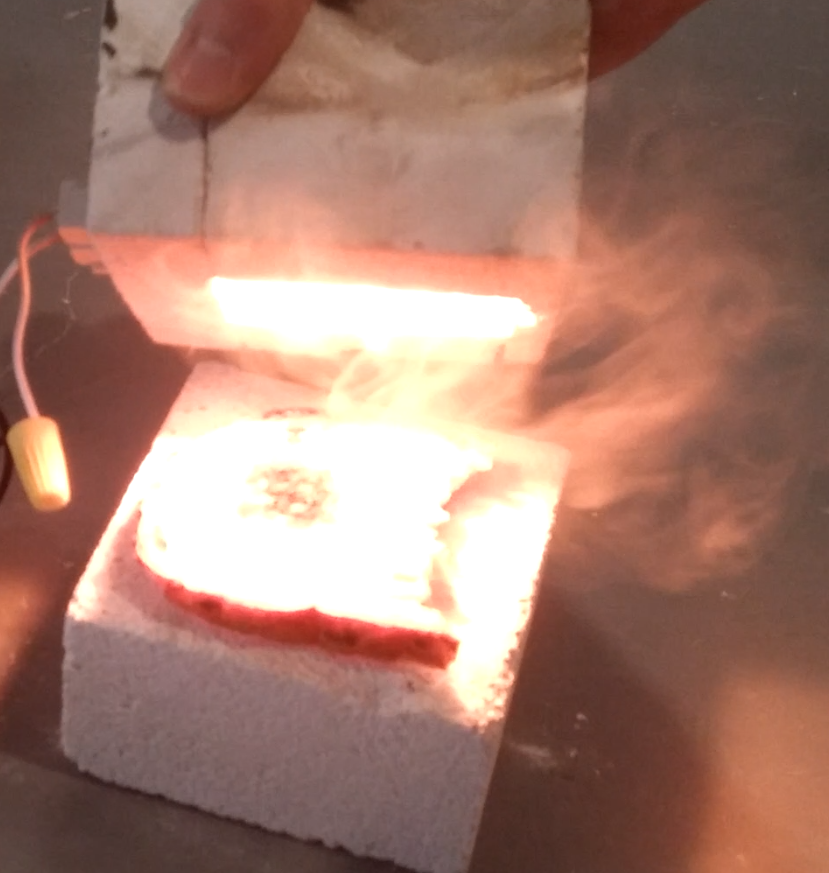
\includegraphics[width=0.5\textwidth]{kiln2}
	}

\end{figure}


There are some surplus SiC elements on ebay, but in general they require fancy termination 

\begin{figure}[H]
	\centering

		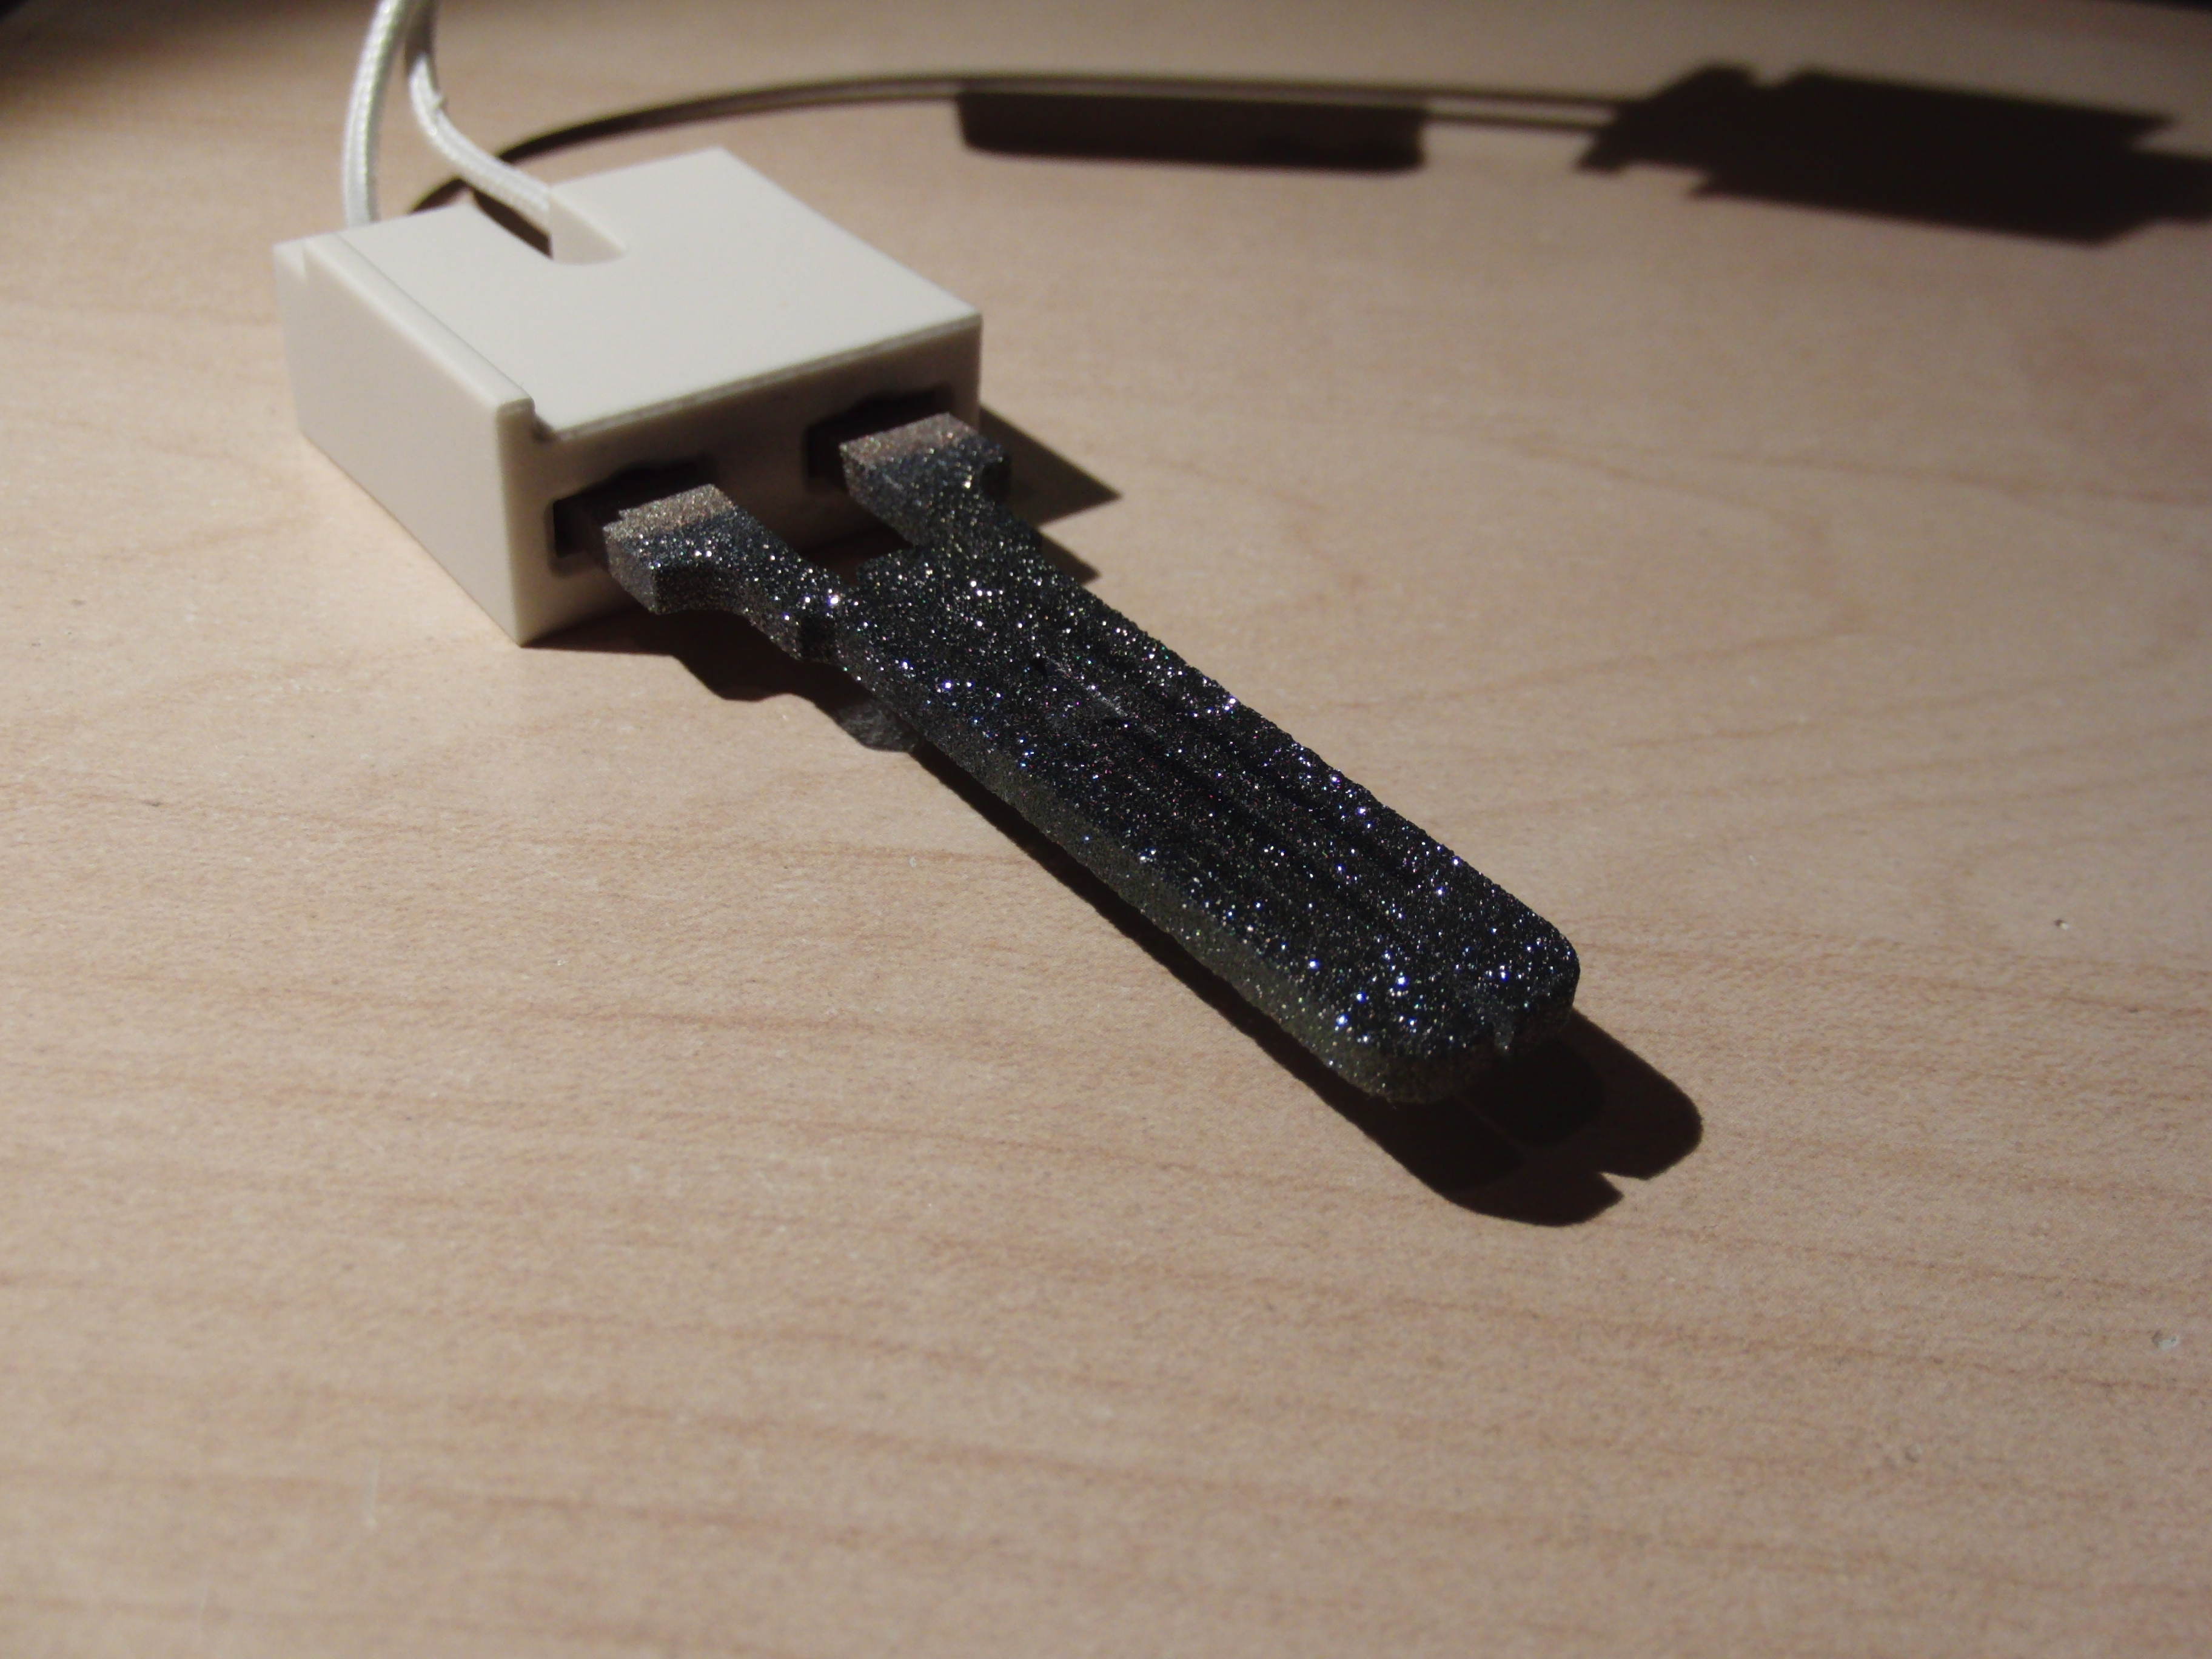
\includegraphics[width=\textwidth]{hsi}
	
	
\end{figure}

This is a hot surface igniter. They're used to ignite gas furnaces for central heating - apparently spark discharges don't have sufficient energy to reliably ignite gas over decades. As of a few years ago (pre-pandemic), they sold for about \$30 on Amazon.

These are an excellent commodity source of SiC elements for ultra-high-temp furnaces. Both SiC and SiNi HSIs are available; SiC greatly preferred due to higher temperature resistance. SiNi HSIs also often specify an 80v DC supply for reasons unknown.



It should be possible to use something like HOOMD-Blue to determine the crystal structure after 

# Ceramics as she is spoke

[References](./references.pdf) | [BibTeX](./bibtex.bib) 



If you don't feel like perusing my prolonged prose (I don't blame you):

1. $30 "hot surface igniters" for gas heaters are made from silicon carbide, and can hit ~1800c - perfect for sintering.
2. PVA-bound alumina with a small amount of Kaolin added to depress sinter point, with Borax crosslinking, cast in machinable wax. See *Cross-linked Polyvinyl Alcohol as a Binder for Gelcasting and Green Machining*, Chabert et al.



==This is a work-in-progress.== The author will likely be unable to proceed for several months, and therefore thought it best to publish this in its current, unfinished state. Remaining tasks:

- Repair kiln.
- Tune mix ratios and characterize the resultant materials.
- Confirm borax compatibility.
- Test argon-graphite.
- Test UV crosslinking.



<hr>






![20190518_142932_HDR](assets/20190518_142932_HDR.jpg)

> This is a poor-quality part; much better quality ones have been produced by this method.
>



I cannot say with any confidence that this is an ideal process; it is merely sufficient for the needs of this device.

The recipe below is overcomplicated to a level previously only found in college statistics textbooks: rest assured that the process only takes ~10 minutes, plus a few hours of drying; and all materials and the required kiln can be procured for <$100. It's essentially baking, but with a slightly hotter oven and off-limits confectioneries.



![Screenshot from 2019-06-03 20-11-28](assets/Screenshot from 2019-06-03 20-11-28.png)



No, seriously. It's just baking.



If you're interested in trying this, I highly recommend skimming through the references. This gel-cast process was taken almost verbatim from *Cross-linked Polyvinyl Alcohol as a Binder for Gelcasting and Green Machining*, with a few minor simplifications; a few minutes' reading of the papers linked will probably be more enlightening than this purely empirical nonsense.



#### The base recipe

| % by mass | Material (Supplier)                                          |
| --------- | ------------------------------------------------------------ |
| 86.5      | Alumina powder (*Calcined Alumina*, \$12/kg, *Tucker's Pottery*) |
| 9         | Kaolin powder (\$20/kg, *Amazon.ca*)                         |
|           |                                                              |
| 0.75      | Borax                                                        |
| 3.5       | Lepage White Glue                                            |
| +20-40%   | Water                                                        |



Add 70 or 90% fine Alumina powder (*Calcined Alumina*, \$12/kg, *Tucker's Pottery*) to 30 or 10% by weight Kaolin powder (\$20/kg, *Amazon.ca*), then mix 'til homogeneous. Add 4% by weight PVA white glue (*LePage general purpose white glue/wood glue* known to work, 45 to 70% solids), then 10% water by weight. 

Mix thoroughly until *cursed Parmesan* texture attained, then alternate adding water and mixing until the solution becomes a thick putty. 30g batches are suitable for manual mixing. The liquid seems to evaporate very rapidly; the putty is only workable for a few minutes.

The green is barely usable without a crosslinker; any handling will break it. @chabert suggest 2,5-dimethoxy 2,5-dihydrofuran, but Borax is more readily available - with the downside that thermal decomposition may emit highly toxic boron vapor.

Unfortunately, borate crosslinks are reversed as soon as the solution dries.



Do not inhale dust; wear a respirator.

According to @chabert2008cross, the delicate green is machinable "if due care is taken". Unfortunately, due care appears to include not machining. This is a thoroughly annoying process; 

Molding with pressure is preferable to prevent voids. A three-piece mold of this style:

#### Pressing

![CIMG6681](assets/CIMG6681.JPG)

is required for reliable ejection: the green is too weak to eject with pins. This mold uses two aluminium dies and replaceable 40mm PVC pipe inserts for parallel drying without Amdahl, producing consistent 25g 6mm thick wafers suitable for CNC milling. ~0.4 MPa pressure required for homogeneity; a hydraulic press was used for these parts, but that isn't strictly necessary. See @nptelpressing for die guidelines.

Beware granular jamming; hardened dies seemed to seize easily. I'm not sure how to prevent this.

![CIMG6679](assets/CIMG6679.JPG)

Wax paper is effective for mold release.

Molding can produce a near-net-shape part, but green binder shrinkage (1.2% typ.) will affect final dimensions. Machining dried green stock nulls out this shrinkage, and avoids the nuisance of unreliable molds.

Previous green binders were sensitive to variations in cross section; differential drying and shrinkage across thin geometries would cause cracking. PVA seems insensitive to these issues. 

Dry for 3-5 hours at ambient. The green is delicate, handle carefully. CNC machine at essentially any reasonable feed/speed; machining properties seem to be similar to graphite. Cutting forces can be surprisingly high at >400m/min surface speeds, so a PLA clamp was used to hold the wafer.

![20190528_210001_HDR](assets/20190528_210001_HDR.jpg)

*Do not inhale dust.* There is some evidence that it will give you Alzheimer's. Dust is highly abrasive, so ensure that axis guards are in place if available and expect dulled tooling.

Uncrosslinked PVA hardens purely by dehydration, so failed mold shots or tailings can be reconstituted with water and added to future batches. 



Sinter at >1450 C. 70% alumina requires ~10 minutes, 90%, ~30 minutes to a strength suitable for most applications. Do not move green after binder burnout; it has zero strength. Parts with volume $<5mm^3$ can be unreliably but rapidly sintered via propane torch; very frustrating, not at all recommended. 



These temperatures are difficult to achieve with conventional ceramic kilns. *Hot Surface Ignitors* for central heating and gas stoves are an excellent commodity source of SiC elements for ultra-high-temp furnaces. Both SiC and SiNi HSIs are available; SiC greatly preferred due to higher temperature resistance. SiNi HSIs also often specify an 80v DC supply for reasons unknown.

SiC HSIs are mechanically delicate, but seem to tolerate ceramic spall and contamination. 

Use `CoorsTek 271N` (or `Emerson 767A-372`) SiC HSI ($33 CAD, Amazon) or equivalent with fiberglass wire insulation, Steatite C220 or Alumina body, nichrome wire. Beware Teflon insulation. 

Typical ratings: a tepid 980 C at 102v to a positively balmy 1705 C at 132v (@coorstek2017). Expect consistent 3.7A draw over entire temperature range.

![kiln](assets/kiln.png)

Kiln built using single Amaco `28035N` 9" by 4-1/2" by 2-1/2" firebrick ($15, Amazon) cut and pocketed using a wet tile saw; the element was then mounted with fire-cement (*Imperial High-Temp Stove and Furnace Cement*). Let cement dry overnight, then slowly raise temperature over course of ~30 minutes. 

The alumina-foam firebrick is quite delicate, and the end-cap to which the element was mounted later broke during handling. Mounting with threaded rods and large washers is recommended.

Depending on local line voltage and alumina purity, a variac may be required to raise voltage ~15% to reach a suitable sinter temperature. 

I have a serious crush on this furnace. It typically reaches 1000c in one minute, and ~1400c in the next two, allowing for very rapid iterative testing (useful for my crude, blunderbuss style of R&D). It can also toast bread in 2.4 seconds. Some green binders (gelatine, specifically) were sensitive to temperature ramp rate; PVA seems unfazed by these crazy dT/dts. 

Bread is not unfazed.

![kiln2](assets/kiln2.png)

Expect element lifespan on the order of ~500 minutes at 130v: degradation occurs via a fascinating two-step interfacial oxidation reaction that evolves carbon monoxide and inflates large bubbles of SiO2 (if I'm understanding @raj2015 correctly - unlikely, given my chemistry prowess):

![my_photo-bubble4](assets/my_photo-bubble4.jpg)

Interestingly, the same "bubbling" failure mode is seen on the reinforced-carbon-carbon panels on the  leading edges of the space shuttle, which are coated with SiO and SiC for oxidation protection. 

This carbon-carbide conversion coating seems to be easy to perform in a furnace such as this one; see Tonsil 5 for details. SiC elements are also used on the ALQ-144 IR missile jammer, so it's unlikely that my laboratory will be hit with a missile in the near future.



A PID control system can be added with an SSR: P: 1, I: 1, D: 2 to 6 based on thermocouple response, and integral windup limits of -300, 300 seems to be an acceptable starting point.



![test_2](assets/test_2.png)



Simple K-type thermocouple wire can operate briefly at 1300c; McMaster-Carr's #3859K44 thermocouples survive 1400c for a few seconds before being incinerated, though the high thermal mass leads to a ~200 C offset in this application (seen in the graph above).

A thin tungsten wire works well as a thermistor, but is rapidly oxidized. Nichrome also works well as a thermistor, though some brands seem to have a strange bijective resistivity curve. It is also destroyed in short order. 

Non-contact temperature measurement is more suitable, though all COTS bolometers begin to whimper at these temperatures. A disappearing-filament pyrometer is trivial to build; if a spectrometer is available, fitting the pleasant glow of the furnace to the Stefan-Boltzmann law can get you within a few hundred degrees. 

A ratio pyrometer built from two photodiodes (or phototransistors, depending on your bias) with IR-cut and IR-pass filters may also work. These techniques are complicated somewhat by alumina's selective radiation: the spectral emissivity curve looks like someone put overcooked pasta into Matplotlib.[^2] Worse still, it varies with temperature by about half an order of magnitude.  

All of this is for naught, however, since active control does not appear to be required with PVA. It appears that parts with repeatable properties can be made as long as the temperature is greater than the sinter point for sufficient time. The pause at 350c for binder burnout mentioned in @chabert2008cross did not seem to be necessary.



This process is not ideal for production: FAST/SPS has several advantages, including full-density sintering at only 1150c, and *as yet there's no consensus as to how it works*. It is *magic*. See @guillon2014field. Thanks to @ice9 for the tip! 



Expect extremely low outgassing (even to LIGO standards), low permeability, continuous service temp ~1500c (with 90% mix - 70% mix became brittle at ~1600c), strength comparable to aluminum (with 70% mix - 90% mix is a little weaker), 20 MV/m breakdown at ambient, hardness Mohs ~9. 

At low temperatures, you can expect extremely low outgassing (even to LIGO standards).

The alumina itself is not an outgassing concern; if you have success with purer alumina compositions, you can expect good vacuum performance all the way to ~1700c. 

The clay binder is a somewhat different story. Pure Kaolin becomes Mullite above 1400c, which is as stable as alumina at low temperatures. However, silica impurities in the Kaolin may begin to sublimate to SiO at above 1300c. See @krieger1965thermodynamics for details; but in general, operation at above ~1400c is contraindicated.

Fired shrinkage values will be added soon.



![temperature](assets/temperature-1559057994888.png)

> *Serves 12: bake till golden brown, then turn over.*



Apologies for the terse and hasty verbiage.

Post improvements or replication at <https://github.com/0xDBFB7/ceramic>, or hit me up @0xDBFB7 on Twitter!

❤





#### Tonsil 1: Brazing

Alumina can be readily brazed by the "active metal" process. In essence, this merely requires a titanium interface layer; the titanium adheres strongly to the alumina when molten, after which standard filler rods and brazing techniques can be used. The entire process must take place in a high vacuum or exceptionally clean argon atmosphere, else inert titanium oxides and nitrides will form. 

A low-melting-point titanium alloy is usually used, as pure Ti melts at some 1800 C. 

A soft copper or Kovar interface layer is often used to prevent differing thermal coefficients from cracking the ceramic when the weld cools. 

See @hammond1988brazing and *Is it possible to braze ceramics?* *P.M.Roberts/Delphi Brazing Consultants* for details.

#### Tonsil 2: $MnO_2$

*Vitreous high alumina porcelain*, @luks1942vitreous, describes how Manganese Dioxide can be used to depress the sinter point of pure alumina to more reasonable temperatures, sometimes without the use of silica. An impure, graphite-contaminated $MnO_2$ can be obtained from alkaline batteries; unfortunately, I was not able to reproduce this effect to any degree.

#### Tonsil 3: Alternative binders

Almost any organic binder can be used.

#### Tonsil 4: Conductive graphite-impregnated 



#### Tonsil 3: Cataphoresis

The initial solution can be thinned considerably, and various objects can be dipped to form hard coatings. Attempts with graphite and aluminum have been successful; however, obtaining a uniform, tight-tolerance layer is somewhat difficult. 

If such a layer is required, a variant of electrophoresis can be used; see @lazic2004influence for details. This technique is often used to insulate indirectly heated cathodes.

#### Tonsil 4: Beta-alumina

Alumina can be found in two main allotropes: alpha-, and beta-. (well, and sapphire, but whatever).

To my (surely flawed) understanding, the chief difference lies in the ionic conductivity, which allows for hermetic low-temperature anodic bonds to some materials using the esoteric Johnsen–Rahbek effect. See Field-Assisted Bonding of Beta-Alumina to Metals, @dunn1979field.

#### Tonsil 5: Foam

If a thin gelatine binder is used in a sol-gel, the solution can be beaten like egg white into a low density insulating foam. I don't know what this is useful for, but it's neat.

#### Tonsil 6: Fire

![temperature](assets/propane.png)

> not sufficiently hot

![acetylene](assets/acetylene-1559058051640.png)

> barely sufficiently hot



[^baking]: Is that how baking works? I don't know. I once substituted 3 cups of salt for sugar in a cake.

[^2]: Disappointed that 'spectral emissivity' has nothing to do with ghosts.





#### Tonsil 7: Applied failure

Almost 8 months of trial and error was required to obtain a usable part by this process. Gel-casting is very well described in the literature and commonly applied in industry.  Here are a few notable failures.



![20181212_182634_HDR](assets/20181212_182634_HDR.jpg)



![20181122_212237_HDR](assets/20181122_212237_HDR.jpg)

> A lost-PLA test with alternate high-temp sol-gel gelatine binder. The mold was filled 





![20181122_222823_HDR](assets/20181122_222823_HDR.jpg)

> Staged firing of less strenuous geometry with same sol-gel process A in low-temp ceramics kiln. These looked amazing, but crumbled to dust upon handling.





> An early propane Bunsen test with gelatine binder, lost-PLA mold, tungsten supports. The A, B, C, and D mixtures shown were 100% alumina, 20% MnO2, 3% porcelain slip, and 10% porcelain slip, respectively.
>
> This was a complete failure on all counts.

![Screenshot from 2019-02-10 15-27-45](assets/Screenshot from 2019-02-10 15-27-45.png)

> Acetylene-sintered with 3% slip.



![20190528_210001_HDR](assets/20190528_210001_HDR-1561693380584.jpg)





\end{document}